
\documentclass[a4paper,14pt]{extarticle}

\usepackage{pythontex}

% for ability to highlight\select and copy text from result pdf output to
% clipboard
\usepackage{cmap}

\usepackage{comment}

\usepackage{setspace}

\usepackage[labelsep=period]{caption}

\usepackage{graphicx}
\graphicspath{ {figure/} }

\usepackage{float}

\usepackage[T2A]{fontenc}
\usepackage[utf8]{inputenc}
\usepackage[russian]{babel}

\usepackage[a4paper,margin=1cm,footskip=1cm,left=2cm,right=1.5cm,top=1.5cm,
		bottom=2cm]{geometry}

\usepackage{textcase}
\usepackage{csquotes}
\usepackage{enumitem}

\usepackage[nottoc]{tocbibind}

% do not show section numbers
%\usepackage[raggedright]{titlesec}

\usepackage{amsmath}

% indent first paragraph in every section
\usepackage{indentfirst}

\usepackage{secdot}

\usepackage[titletoc,title]{appendix}


% indent description items
\setlist[description]{leftmargin=\parindent,labelindent=\parindent}

% ?
%\patchcmd{\appendices}{\quad}{: }{}{}

\setcounter{secnumdepth}{3}
\setstretch{1.5}

\DeclareMathOperator{\Sp}{Sp}

\let\oldref\ref
\renewcommand{\ref}[1]{(\oldref{#1})}

\begin{document}

\begin{titlepage}

	\begin{center}
		\MakeTextUppercase{Министерство образования и науки Российской~Федерации}

		\bigbreak

		ФЕДЕРАЛЬНОЕ ГОСУДАРСТВЕННОЕ БЮДЖЕТНОЕ ОБРАЗОВАТЕЛЬНОЕ УЧРЕЖДЕНИЕ
			ВЫСШЕГО ОБРАЗОВАНИЯ

		\bigbreak

		\MakeTextUppercase{\enquote{Новосибирский государственный технический
			университет}}
		\vspace{5pt}
		\hrule

		\bigbreak

		Кафедра теоретической и прикладной информатики

		\vspace{50pt}

		\textbf{\LARGE{Отчет по}\\}

		\bigbreak

		производственной практике: \\
			практике по получению профессиональных умений и опыта профессиональной
			деятельности

		\bigbreak

		c 1 ноября по 31 декабря

		\bigbreak

		<<Параметрическая идентификация стохастических динамических линейных
		непрерывно-дискретных систем>>

		\vspace{50pt}

	\end{center}

	\begin{flushleft}
		\begin{tabbing}
			Группа:\qquad\qquad\qquad \= ПММ-61\\
			Студент:                  \> Горбунов К. К.\\
			Место практики:           \> отдел № 8 ФГУП <<СНИИМ>> \\
			Руководитель:             \> нач. отдела № 8, Толстиков А.С.
		\end{tabbing}
	\end{flushleft}

	\begin{center}
		\vspace{\fill}
		Новосибирск, 2016 г.
	\end{center}

\end{titlepage}

\tableofcontents

\newpage

\section*{Введение}
\addcontentsline{toc}{section}{Введение}

В настоящее время математическое моделирование играет фундаментальную роль в
науке и технике и является одним из интенсивно развивающихся перспективных
научных направлений в области информатики.

Проблема идентификации, связанная с построением математических моделей по
экспериментальным данным, относится к одной из основных проблем теории и
практики автоматического управления. Ее качественное решение способствует
эффективному применению на практике современных математических методов и
наукоемких технологий, например, при расчете и проектировании систем управления
подвижными (в том числе авиационно-космическими) и технологическими объектами,
построении прогнозирующих моделей (например, в экономике и бизнес-процессах),
конструировании следящих и измерительных систем \cite{denisov}.

\section{Постановка задачи}

\subsection[Структурно-вероятностное описание модельной структуры]
{Структурно-вероятностное описание модельной \\структуры}

% remember to measure identification accuracy in spaces of outputs and
% parameters
%\noindent $\frac{||\theta^* -\ \hat{\theta}||}{||\theta^*||}$
%\\
%\\
%$\frac{||y^* -\ \hat{y}||}{||y^*||}$
%\\
\renewcommand{\vec}[1]{\mathbf{#1}}

Определим модель стохастической динамической линейной \\непрерывно-дискретной
системы в простанстве состояний в общем виде:
\begin{equation}
	\label{eq:initmod}
	\left\{ 
		\begin{array}{lll}
			\frac{d}{dt}x(t) &= F(\theta) \vec{x}(t) + C \vec{u}(t) + G \vec{w}(t),
				& t \in [t_0,T] \\ 
			\vec{y}(t_k)           &= H \vec{x}(t_k) + \vec{v}(t_k), 
				& k = 1,\ldots, N
		\end{array} 
	\right. 
\end{equation}

Здесь:
\begin{description}
	\item [$\vec{x}(t_k)$] -- вектор состояния;
	\item [$F$] -- матрица перехода состояния;
	\item [$\vec{u}(t_k)$] -- вектор-функция управления (входного воздействия);
	\item [$C$] -- матрица управления;
	\item [$\vec{w}(t_k)$] -- вектор возмущений;
	\item [$G$] -- матрица влияния возмущений;
	\item [$H$] -- матрица наблюдения;
	\item [$\vec{v}(t_k)$] -- шум измерений;
	\item [$\vec{y}(t_k)$] -- вектор наблюдений (измерений) отклика;
\end{description}

В данной модели уравнение объекта является непрерывным, а уравнение наблюдений
--- дискретным. Такая модель является характерной для значительного множества
прикладных задач.

Одной из целей исспедований в рамках магистерской диссертации является
разработка алгоритмов оценивания состояния и идентификации стохастической 
динамической непрерывно-дискретной модели вида \ref{eq:initmod}. 

Один из видимых путей решения задачи оценивания состояния такой системы
является адаптация аналогичных алгоритмов, применимых к дискретным и
непрерывным системам, к данному непрерывно-дискретному случаю.

Разрабатываемый алгоритм также должен оценивать вероятностные характеристики
шумов объекта и измерений, потому как в реальных задачах вероятностные
характеристики данных процессов неизвестны или же эти процессы являются
нестационарными.

\section[Параметрическая идентификация моделей стохастических
\\непрерывно-дискретных систем]
{Параметрическая идентификация моделей \\стохастических
непрерывно-дискретных систем} 

Идентификацией динамической системы называется определение структуры и
параметров математической модели, обеспечивающих наилучшее совпадение выходных
переменных моделей переменных модели и системы при одинаковых входных
воздействиях \cite{chubich}.

Под параметрической идентификацией, в частности, понимается только определение
параметров модели. Предполагается, что структура модели известна.

В данной работе в качестве критерия идентификации используется критерий
максимального правдоподобия, а получаемые оценки параметров модели является
оценками максимального правдоподобия (ОМП).

\subsection{Вычисление значения критерия идентификации}

\newcommand{\eps}{\varepsilon}

Выражение для критерия максимального правдоподобия имеет вид \cite{denisov}:
\begin{equation}
\begin{split}
\chi(\theta) = -\ln{L(Y_1^N;\theta)} = \frac{Nm}{2} \ln{2\pi} +
\\ + \frac{1}{2} \sum\limits_{k=1}^{N} 
\left[ \eps^T(t_k, \theta) B^{-1}(t_k, \theta) \eps(t_k, \theta) + 
\ln \det B(t_k, \theta) \right].
\end{split}
\end{equation}

Здесь:

\begin{description}
\item[$Y_1^N$] --- множество из $N$ наблюдений отклика
\item[$\theta$] --- вектор параметров модели 
\item[$\chi(\cdot)$] --- функционал, используемый в качестве критерия
идентификации
\item[$L(\cdot)$] --- функционал максимального правдоподобия 
\item[$N$] --- число дискретных моментов времени наблюдений
\item[$m$] --- число выходных каналов системы (размерность вектора наблюдений
отклика)
\item[$\eps(t_j) = y(t_j) - H \hat{x}(t_j|t_{j-1})$] --- обновляющая
последовательность 
\item[$B(t_j) = HP(t_j|t_{j-1})H^T + R$] --- ковариационная обновляющей
последовательности 
\end{description}

\newpage
Алгоритм вычисления значения критерия следующий:

\begin{enumerate}
\item Пусть $j = 1$, $\chi(\theta) = 0$.
\item Решаются дифференциальные уравнения непрерывно-дискретного фильтра
Калмана с соответствующими начальными условиями:
\[
\frac{d}{dt}\hat{x}(t|t_{j-1}) = F \hat{x}(t|t_{j-1}) + C u(t),\ 
t_{j-1} \le t \le t_j,\ \hat{x}(t_0|t_0) = \bar{x}_0;
\]
\[
\frac{d}{dt}P(t_j|t_{j-1}) = F P(t|t_{j-1}) + P(t|t_{j-1}) F^T + GQG^T,\\
\]
\[
t_{j-1} \le t \le t_j,\ P(t_0|t_0) = P_0;
\]
Получаем $\hat{x}(t_j|t_{j-1})$ и $P(t_j|t_{j-1})$.

\item Вычисляются
\[ \eps(t_j) = y(t_j) - H \hat{x}(t_j|t_{j-1}); \]
\[ B(t_j) = H P(t_j|t_{j-1}) H^T + R; \]
\[
K(t_j) = P(t_j|t_{j-1}) H^T B^{-1}(t_j).
\]

\item Вычисляется соответствующая $j$-му моменту времени составляющая функции
правдоподобия (2.35)
\[
S = \frac{1}{2} \left[ B^{-1}(t_j) \eps(t_j) + \ln \det B(t_j) \right].
\]

\item Накапливается сумма
\[
\chi(\theta) = \chi(\theta) + S.
\]

\item Если $j = N$, то
\[
\chi(\theta) = \chi(\theta) + \frac{Nm}{2} \ln 2\pi
\]
и вычисления прекращаются, иначе --- вычисляются следующие начальные условия по
формулам
\[
\hat{x}(t_j|t_{j-1}) = \hat{x}(t_j|t_{j-1}) + K(t_j) \eps(t_j);
\]
\[
P(t_j|t_{j-1}) = \left[ I - K(t_j) H \right] P(t_j|t_{j-1}),
\]
$j$ заменяется на $j+1$ и осуществляется переход на шаг 2.

\end{enumerate}

\subsection[Вычисление значения градиента критерия идентификации]
{Вычисление значения градиента критерия \\идентификации}

В данной работе предлагается к рассмотрению два практических метода вычисления
значения градиента критерия идентификации: по аналитическому выражению и с
использованием программных средств автоматического дифференцирования.

Далее приведено краткое описание каждого из этих методов.

\subsubsection{Вычисление по аналитическому выражению}


Аналитическое выражение производных критерия следующее \cite{denisov}:

\begin{multline}
	\label{eq:llderiv}
	\frac{\partial \chi(\theta)}{\partial \theta_k} = \sum\limits^{N}_{j=1}
	\left[
	\eps^{T}(t_j) B^{-1}(t_j) \frac{\partial \eps(t_j)}{\partial \theta_k} -
	\frac{1}{2} \eps^{T}(t_j) B^{-1}(t_j) \frac{\partial B(t_j)}
	{\partial \theta_k}
	B^{-1}(t_j) \eps(t_j) + \right.\\\left.
	\frac{1}{2}
	\Sp \left( B^{-1}(t_j) \frac{\partial B(t_j)}{\partial \theta_k} \right)
	\right] ,\ k = 1,\ldots,s,
\end{multline}
где $s$ --- размерность вектора неизвестных параметров $\Theta$.

В выражении \ref{eq:llderiv} частные производные $\frac{\partial \eps(t_j)}
{\partial \theta_k}$ и $\frac{\partial B(t_j)}{\partial \theta_k}$ вычисляются
с помощью следующим выражений:
\begin{equation}
\frac{\partial \eps(t_j)}{\partial \theta_k} = - \frac{\partial H}
{\partial \theta_k} \hat{x}(t_j|t_{j-1}) - H \frac{\partial 
	\hat{x}(t_j|t_{j-1})}
{\partial \theta_k},\\
\end{equation}

\begin{equation}
\frac{\partial B(t_j)}{\partial \theta_k} = \frac{\partial H}
	{\partial \theta_k}
P(t_j|t_{j-1}) H^T + H \frac{\partial P(t_j|t_{j-1})}{\partial \theta_k} H^T +
H P(t_j|t_{j-1}) \frac{\partial H^T}{\partial \theta_k} + \frac{\partial R}
{\partial \theta_k}.
\end{equation}

Уравнения чувствительности для оценки вектора состояний:
\begin{multline}
\label{eq:senstate}
\frac{d}{dt}
\begin{bmatrix}
	\hat{x}(t|t_{j-1}) \\
	\frac{\partial \hat{x}(t|t_{j-1})}{\partial \theta_1} \\
	\vdots \\
	\frac{\partial \hat{x}(t|t_{j-1})}{\partial \theta_s}
\end{bmatrix} =
\begin{bmatrix}
	F \hat{x}(t|t_{j-1}) + G u(t) \\
	\frac{\partial F}{\partial \theta_1} \hat{x}(t|t_{j-1}) +
		F \frac{\partial \hat{x}(t|t_{j-1})}{\partial \theta_1} +
		\frac{\partial G}{\partial \theta_1} u(t) \\
	\vdots  \\
	\frac{\partial F}{\partial \theta_s} \hat{x}(t|t_{j-1}) +
		F \frac{\partial \hat{x}(t|t_{j-1})}{\partial \theta_s} +
		\frac{\partial G}{\partial \theta_s} u(t)
\end{bmatrix} = \\ =
\begin{bmatrix}
	F & 0 & \cdots & 0 \\
	\frac{\partial F}{\partial \theta_1} & F & \cdots & 0 \\
	\vdots & \vdots & \ddots & \vdots \\
	\frac{\partial F}{\partial \theta_s} & 0 & \cdots & F
\end{bmatrix} \cdot
\begin{bmatrix}
	\hat{x}(t|t_{j-1}) \\
	\frac{\partial \hat{x}(t|t_{j-1})}{\partial \theta_1} \\
	\vdots \\
	\frac{\partial \hat{x}(t|t_{j-1})}{\partial \theta_s} \\
\end{bmatrix} +
\begin{bmatrix}
	G \\
	\frac{\partial{G}}{\partial \theta_1} \\
	\vdots \\
	\frac{\partial{G}}{\partial \theta_s}
\end{bmatrix} u(t),\\
\hspace{\fill} t_{j-1} \le t \le t_j,\ j=1,\ldots,N. \hspace{\fill}
\end{multline}

Начальные условия:
\begin{itemize}

\item для $j = 1$

\begin{equation}
\label{eq:senstateinitcond1}
\begin{bmatrix}
	\hat{x}(t_0|t_0) \\
	\frac{\partial \hat{x}(t_0|t_0)}{\partial \theta_1} \\
	\vdots \\
	\frac{\partial \hat{x}(t_0|t_0)}{\partial \theta_s}
\end{bmatrix} =
\begin{bmatrix}
	\overline{x_0} \\
	\frac{\partial \overline{x_0}}{\partial \theta_1} \\
	\vdots \\
	\frac{\partial \overline{x_0}}{\partial \theta_s}
\end{bmatrix}
\end{equation}

\item для $j = 2, 3, \ldots, N$

\begin{equation}
\label{eq:senstateinitcondj}
\begin{bmatrix}
	\hat{x}(t_j|t_j) \\
	\frac{\partial \hat{x}(t_j|t_j)}{\partial \theta_1} \\
	\vdots \\
	\frac{\partial \hat{x}(t_j|t_j)}{\partial \theta_s}
\end{bmatrix} =
\begin{bmatrix}
	\hat{x}(t_j|t_{j-1}) + K(t_j) \eps(t_j) \\
	\frac{\partial \hat{x}(t_j|t_{j-1})}{\partial \theta_1} + 
	\frac{\partial K(t_j)}
		{\partial \theta_1} \eps(t_j) + K(t_j) \frac{\partial \eps(t_j)}
		{\partial \theta_1} \\
		\vdots \\
	\frac{\partial \hat{x}(t_j|t_{j-1})}{\partial \theta_s} + 
	\frac{\partial K(t_j)}
		{\partial \theta_s} \eps(t_j) + K(t_j) \frac{\partial \eps(t_j)}
		{\partial \theta_s}
\end{bmatrix}.
\end{equation}

\end{itemize}

Уравнения чувствительности для ковариационной матрицы оценки вектора состояний:
\begin{multline}
	\label{eq:senscov}
	\frac{d}{dt}
	\begin{bmatrix}
		P(t|t_{j-1}) \\
		\frac{\partial P(t|t_{j-1})}{\partial \theta_1} \\
		\vdots \\
		\frac{\partial P(t|t_{j-1})}{\partial \theta_s}
	\end{bmatrix} = \\
	= \begin{bmatrix}
		F P(t|t_{j-1}) + P(t|t_{j-1}) F^T + G Q G^T \\
		\frac{\partial F}{\partial \theta_1} P(t|t_{j-1}) +
			F \frac{\partial P(t|t_{j-1})}{\partial \theta_1} +
			\frac{\partial P(t|t_{j-1})}{\partial \theta_1} F^T + \hspace{\fill} \\
			\hspace{8em} + P(t|t_{j-1}) \frac{\partial F^T}{\partial \theta_1} +
			\frac{\partial G}{\partial \theta_1} Q G^T +
			G \frac{\partial Q}{\partial \theta_1} G^T +
			G Q \frac{\partial G^T}{\partial \theta_1} \\
		\vdots \\
		\frac{\partial F}{\partial \theta_s} P(t|t_{j-1}) +
			F \frac{\partial P(t|t_{j-1})}{\partial \theta_s} +
			\frac{\partial P(t|t_{j-1})}{\partial \theta_s} F^T + \hspace{\fill} \\
			\hspace{8em} + P(t|t_{j-1}) \frac{\partial F^T}{\partial \theta_s} +
			\frac{\partial G}{\partial \theta_s} Q G^T +
			G \frac{\partial Q}{\partial \theta_s} G^T +
			G Q \frac{\partial G^T}{\partial \theta_s}
	\end{bmatrix}  = \\
	= \begin{bmatrix}
		F & 0 & \cdots & 0 \\
		\frac{\partial F}{\partial \theta_1} & F & \cdots & 0 \\
		\vdots & \vdots & \ddots & \vdots \\
		\frac{\partial F}{\partial \theta_s} & 0 & \cdots & F \\
	\end{bmatrix}
	\begin{bmatrix}
		P(t|t_{j-1}) \\
		\frac{\partial P(t|t_{j-1})}{\partial \theta_1} \\
		\vdots \\
		\frac{\partial P(t|t_{j-1})}{\partial \theta_s}
	\end{bmatrix} +
	\begin{bmatrix}
	P(t|t_{j-1}) & 0 & \cdots & 0 \\
	\frac{\partial P(t|t_{j-1})}{\partial \theta_1} & P(t|t_{j-1}) & \cdots & 0 \\
	\vdots & \vdots & \ddots & \vdots \\
	\frac{\partial P(t|t_{j-1})}{\partial \theta_s} & 0 & \cdots & P(t|t_{j-1})
	\end{bmatrix}
	\begin{bmatrix}
		F^T \\
		\frac{\partial F^T}{\partial \theta_1} \\
		\vdots \\
		\frac{\partial F^T}{\partial \theta_s}
	\end{bmatrix} + \\
	+ \begin{bmatrix}
		G Q G^T\\
		\frac{\partial G}{\partial \theta_1} Q G^T \\
		\vdots \\
		\frac{\partial G}{\partial \theta_s} Q G^T
	\end{bmatrix} +
	\begin{bmatrix}
		0 \\
		G \frac{\partial Q}{\partial \theta_1} G^T \\
		\vdots \\
		G \frac{\partial Q}{\partial \theta_s} G^T
	\end{bmatrix} +
	\begin{bmatrix}
		0 \\
		G Q \frac{\partial G^T}{\partial \theta_1} \\
		\vdots \\
		G Q \frac{\partial G^T}{\partial \theta_s}
	\end{bmatrix},\\ \hspace{\fill} t_{j-1} \le t \le t_j, \quad j = 1, \ldots, N. \hspace{\fill}
\end{multline}

\newpage
Начальные условия:
\begin{itemize}

	\item для $j = 1$

\begin{equation}
\label{eq:senscovinitcond1}
\begin{bmatrix}
	P(t_0|t_0) \\
	\frac{\partial P(t_0|t_0)}{\partial \theta_1} \\
	\vdots \\
	\frac{\partial P(t_0|t_0)}{\partial \theta_s}
\end{bmatrix} =
\begin{bmatrix}
	P_0 \\
	\frac{\partial P_0}{\partial \theta_1} \\
	\vdots \\
	\frac{\partial P_0}{\partial \theta_s}
\end{bmatrix}
\end{equation}

\item для $j = 2, 3, \ldots, N$

\begin{multline}
\label{eq:senscovinitcondj}
\begin{bmatrix}
	P(t|t_j) \\
	\frac{\partial P(t_j|t_j)}{\partial \theta_1} \\
 	\vdots \\
	\frac{\partial P(t_j|t_j)}{\partial \theta_s}
\end{bmatrix} =
\begin{bmatrix}
	\left\{ I - K(t_j) H \right\} P(t_j|t_{j-1}) \\
	\left[ - \frac{\partial K(t_j)}{\partial \theta_1} H - K(t_j)
		\frac{\partial H}{\partial \theta_1} \right] P(t_j|t_{j-1}) + 
		\left\{ I - K(t_j) H \right\}
		\frac{\partial P(t_j|t_{j-1})}{\partial \theta_1} \\
	\vdots \\
	\left[ - \frac{\partial K(t_j)}{\partial \theta_s} H - K(t_j)
		\frac{\partial H}{\partial \theta_s} \right] P(t_j|t_{j-1}) + 
		\left\{ I - K(t_j) H \right\}
		\frac{\partial P(t_j|t_{j-1})}{\partial \theta_s} \\
\end{bmatrix},
\end{multline}

\end{itemize}

где
\begin{multline}
	\frac{\partial K(t_j)}{\partial \theta_k} =
		\frac{\partial P(t_j|t_{j-1})}{\partial \theta_k} H^T B^{-1}(t_j) + 
		P(t_j|t_{j-1}) \frac{\partial H^T}{\partial \theta_k} B^{-1}(t_j) - \\ -
		P(t_j|t{j-1}) H^{-1} B^{-1}(t_j) \frac{\partial B(t_j)}{\partial \theta_k}
		B^{-1}(t_j).
\end{multline}

Алгоритм может быть следующим:

\begin{enumerate} 

\item $j = 1$,\enskip $\frac{\partial \chi (\theta)}{\partial \theta_k} = 0$,
 \enskip $k = 1, \ldots, s$,\quad где $s$ --- размерность вектора \\ параметров
 $\Theta$.

\item Решаются уравнения чувствительности для оценки вектора состояния
\ref{eq:senstate} и его ковариационной матрицы \ref{eq:senscov} с начальными
условиями \ref{eq:senstateinitcond1} и \ref{eq:senscovinitcond1}
соответственно. Получаем $\hat{x}(t_j|t_{j-1})$ и $P(t_j|t_{j-1})$.

\item Вычисляются
\[
	B(t_j) = H P(t_j|t_{j-1}) H^T + R;
\]
\begin{multline}
	\frac{\partial B(t_j)}{\partial \theta_k} =
		\frac{\partial H}{\partial \theta_k} P(t_j|t_{j-1}) H^T + H
		\frac{\partial P(t_j|t_{j-1})}{\theta_k} H^T + \\ +
		H P(t_j|t_{j-1}) \frac{\partial H^T}{\partial \theta_k} +
		\frac{\partial R}{\partial \theta_k},\qquad k = 1, \ldots, s.
\end{multline}

\newcommand{\pd}[2]{\frac{\partial #1}{\partial #2}}

\item Вычисляются
\[
	K(t_j) = P(t_j|t_{j-1}) H^T B^{-1}(t_j);
\]
\begin{multline}
	\pd{K(t_k)}{\theta_i} = \pd{P(t_k|t_{k-1})}{\theta_i} H^T B^{-1}(t_k) +
	P(t_k|t_{k-1}) \pd{H^T}{\theta_i} B^{-1}(t_k) - \\
	- P(t_k|t_{k-1}) H^T B^{-1}(t_k)
	\pd{B(t_k)}{\theta_i} B^{-1}(t_k),\qquad i = 1, \ldots, s.
\end{multline}

\item Вычисляются
\[
	\eps(t_j) = y(t_j) - H \hat{x}(t_j|t_{j-1});
\]
\[
	\pd{\eps(t_j)}{\theta_k} = - \pd{H}{\theta_k} \hat{x}(t_j|t_{j-1}) -
		H \pd{\hat{x}(t_j|t_{j-1})}{\theta_k},\qquad k = 1, \ldots, s.
\]

\item Вычисляется соответствующая $j$-му моменту времени составляющая градиента
функции правдоподобия \ref{eq:llderiv}
\begin{multline}
	S(k) = \eps^T(t_j) B^{-1}(t_j) \pd{\eps(t_j)}{\theta_k} - \frac{1}{2}
	\eps^T(t_j) B^{-1}(t_j) \pd{B(t_j)}{\theta_k} B^{-1}(t_j) \eps(t_j) + \\ +
	\frac{1}{2} \Sp{ B^{-1}(t_j) \pd{B(t_j)}{\theta_k} },\qquad k = 1, \ldots, s.
\end{multline}

\item Накапливается сумма
\[
	\pd{\chi(\theta)}{\theta_k} = \pd{\chi(\theta)}{\theta_k} + S(k),
		\qquad k = 1, \ldots, s.
\]

\item Если $j = N$, то вычисления прекращаются, иначе --- вычисляются следующие
начальные условия по формулам \ref{eq:senstateinitcondj} и
\ref{eq:senscovinitcondj}, $j$ заменяется на $j + 1$, и осуществляется переход
на шаг 2.

\end{enumerate}

\subsubsection{Программный метод автоматического дифференцирования}

Рассматриваемый программный метод берет свое начало из задач машинного обучения
глубоких нейронных сетей, которые в настоящее время являются популярным
объектом научных исследований, образующие целое новое научное направление ---
глубинное обучение (deep learning). Глубокие нейронные сети применяются для
решения широкого класса практических задач распознавания, классификации,
предсказания, обработки и анализа ествесственных языков и многих других.

Глубокими нейронными сетями называются такие сети, которые имеют в своем
составе большое число скрытых слоев нейронов, и, следовательно, суммарно
большое число нейронов.

Задачу обучения нейронной сети можно трактовать как оценивание параметров этой
сети по некоторым полученным извне наборам данных (наблюдениям), которые
называются обучающими наборами данными. Параметрами сети являются веса связей
между её нейронами. Так как по определению глубокой сети число входящих в неё
нейронов велико, то, соответственно, велико и число <<оцениваемых>> параметров
(весов).

В связи с большим числом параметров (весов) возникают проблемы применимости
методов оценивания с использованием традиционных методов вычисления градиента
функции потерь (критерия) для поиска экстремальных значений. Эти проблемы,
связаны, во-первых, с невозможностью вывода аналитического выражения градиента
для модели со столь большим числом параметров (сотни тысяч, миллионы параметров
/ весов) и столь сложной структурой как нейронная сеть. Во-вторых, методы
приближенного вычисления градиента не позволяют достичь удовлетворительной
точности для обеспечения сходимости оптимизационной процедуры к искомому
решению.

Программный метод автоматического дифференцирования или также называемый метод
обратного распространения ошибки основан на правиле дифференцирования сложной
функции --- <<правиле цепи>> (<<chain rule>>), и предполагает определения
производной для каждой операции используемой системы компьютерной алгебры.
Данный метод позволяет вычислять градиент быстро и точно, не программируя явно
его вычисления. Отсюда и название метода --- автоматическое дифференцирование.
Следует отметить, очевидно, что с помощью этого метода также можно вычислять
и производные высших порядков быстро и без потери точности.

\begin{figure}[H]
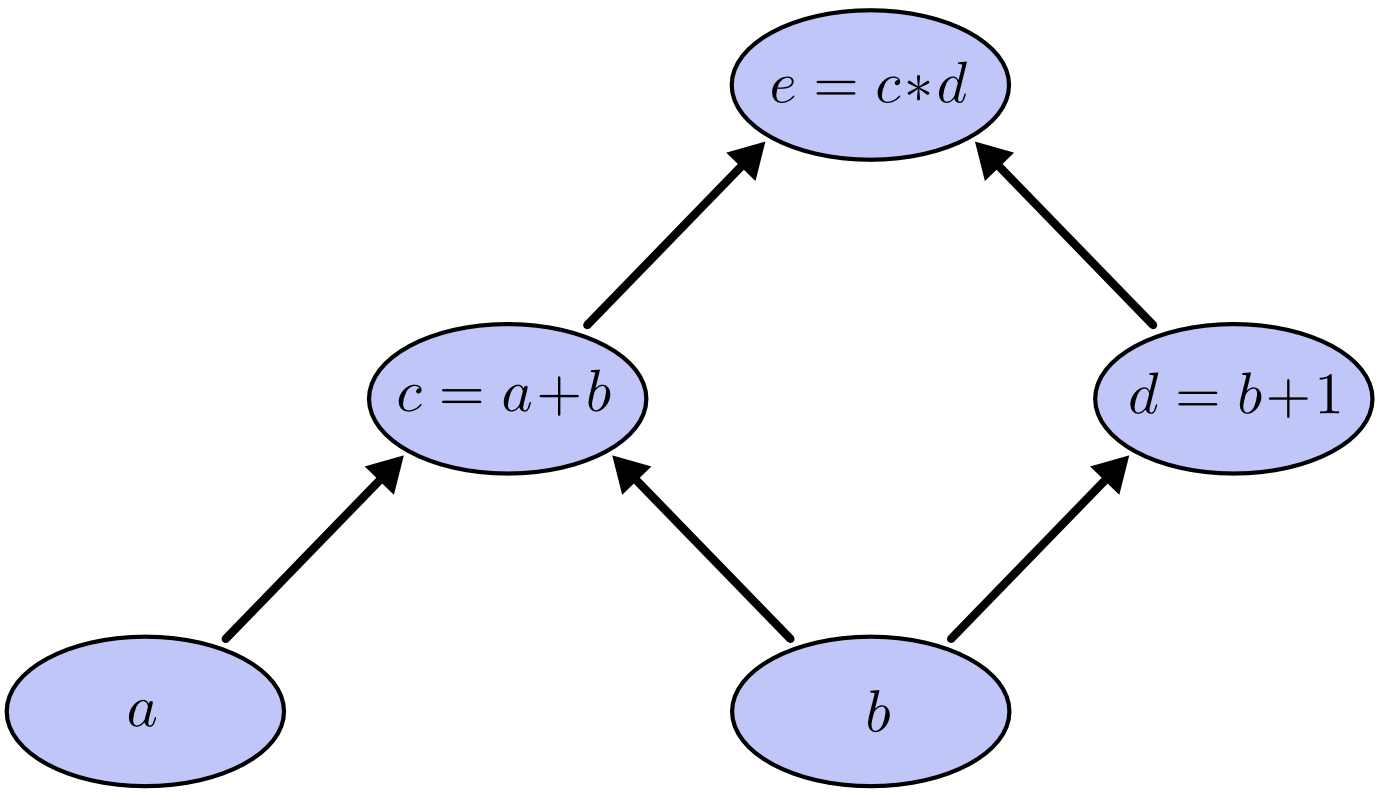
\includegraphics[width=\textwidth]{tree-def}
\caption{Простой пример вычислительного графа \cite{colah}.}
\end{figure}

\begin{figure}[H]
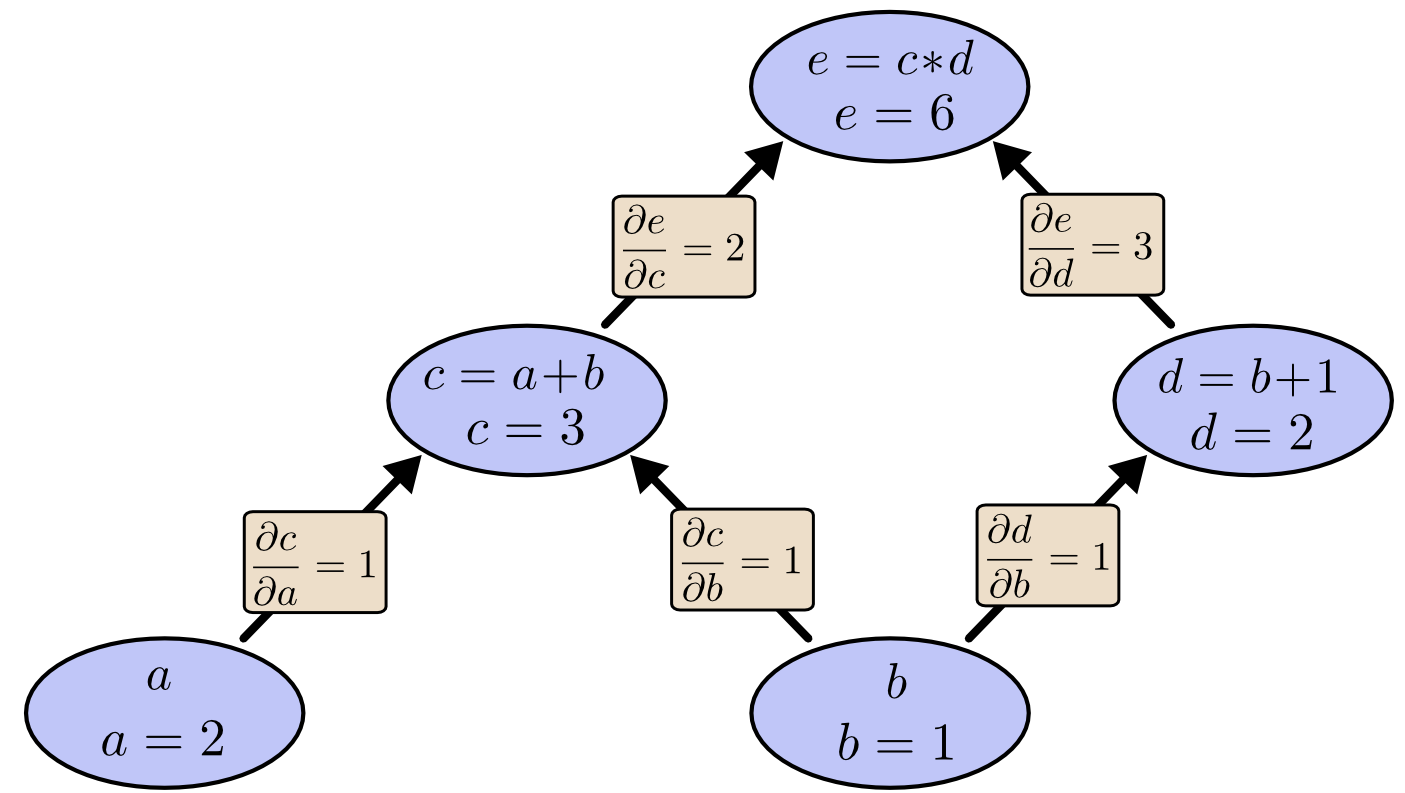
\includegraphics[width=\textwidth]{tree-eval-derivs}
\caption{Пример вычислительного графа с определением производных \cite{colah}.}
\end{figure}

\begin{figure}[H]
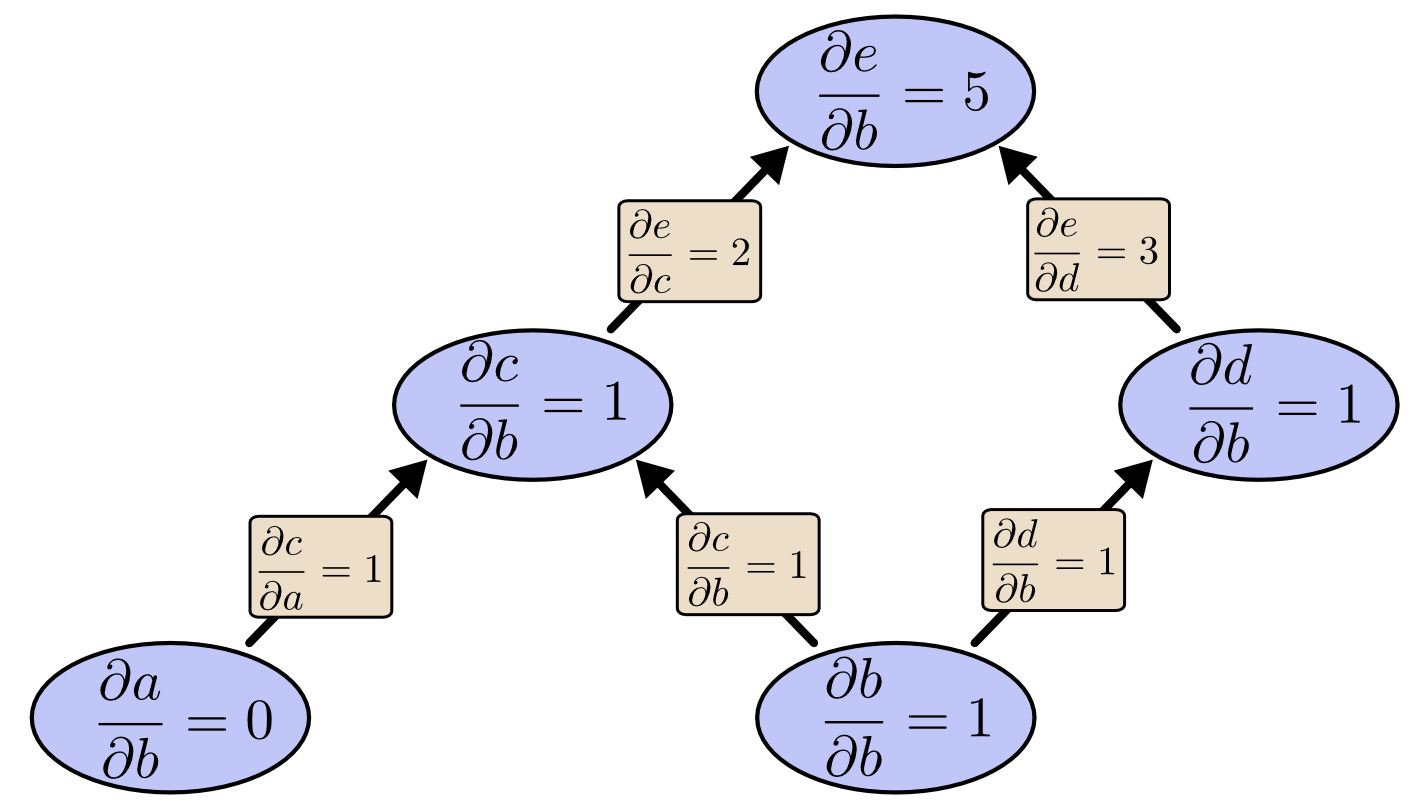
\includegraphics[width=\textwidth]{tree-forwardmode}
\caption{Вычисление произодной графа \cite{colah}.}
\end{figure}

Наиболее популярные системы, в которых реализовано автоматическое
дифференцирование: TensorFlow \cite{tf}, Theano \cite{theano},
Torch\cite{torch}. Существует большое число других систем и средств. В данной
работе используется система TensorFlow.

\subsection{Программные аспекты реализации вычислений}

В данной работе используется библиотека для глубинного машинного обучения и
система компьютерной алгебры TensorFlow. В этой системе всякая вычислительная
программа является ориентированным (вычислительным) графом, в котором вершины
являются операциями или данными, а ребра указывают направления <<движения>>
данных. Основной структурой данных является Tensor --- обобщение скаляров,
векторов-столбцов, строк, квадратных и прямоугольных матриц и вообще любого
многомерного массива. Отсюда и название системы <<TensorFlow>> --- <<поток
тензоров>>.

Программу, использующую TensorFlow, в простейшем случае можно условно разделить
на две части: в первой части определяется вычислительный граф, во второй части
этот граф запускается, исполняется. Создание графа --- процесс относительно
медленный и занимает единицы, а может и десятки секунд, этот процесс можно
сравнить с компиляцией. Зато по успешному завершению созданию графа получаем
быструю, эффективную, параллельную вычислительную программу, которая в
подавляющем большинстве случаев будет превосходить по скорости программы,
написанные за некоторое короткое время с нуля на языке C/С++.

Система TensorFlow использует результаты теории графов и позволяет эффективно 
распараллеливать алгоритмы. К тому же в системе заложен функционал, позволяющий
производить вычисления распределенно, на нескольких машинах.

\newpage
\section[Результаты экспериментальных модельных исследований]
{Результаты экспериментальных модельных \\исследований} 


\subsection{Спецификация модели}
Рассмотрим простую модель второго порядка. 

Число параметров ($\theta_i$) $s = 2$. Параметры являются диагональными
элементами матрицы перехода со знаком ``минус'', ожидание начального состояния
нулевое, все ковариации равны $0.01$, ожидание начального состояния нулевое.
Матрицы управления, наблюдения, влияния шума --- единичные.
\[
	\frac{d}{dt}x(t) =
		\begin{pmatrix}
			-\theta_1 & 0 \\
			0 & -\theta_2
		\end{pmatrix}
		\vec{x}(t) +
		\begin{pmatrix}
			1 & 0 \\
			0 & 0
		\end{pmatrix}
		\vec{u}(t) +
		\begin{pmatrix}
			1 & 0 \\
			0 & 1
		\end{pmatrix}
		\vec{w}(t),
\]
\[
	\vec{y}(t_k) =
	\begin{pmatrix}
		1 & 0 \\
		0 & 1
	\end{pmatrix}
	\vec{x}(t_k) + \vec{v}(t_k),
\]
\[
	\vec{x}(t) = \begin{bmatrix} x_1(t) \\ x_2(t) \end{bmatrix},\ 
	\vec{u}(t) = \begin{bmatrix} u_1(t) \\ u_2(t) \end{bmatrix},\
	\vec{w}(t) = \begin{bmatrix} w_1(t) \\ w_2(t) \end{bmatrix},\
	\vec{y}(t_k) = \begin{bmatrix} y_1(t_k) \\ y_2(t_k) \end{bmatrix},\
\]
\[
	\vec{v}(t_k) = \begin{bmatrix} v_1(t_k) \\ v_2(t_k) \end{bmatrix},\
\]
\[
	R = Q = P_0 = \begin{pmatrix} 0.01 & 0 \\ 0 & 0.01 \end{pmatrix},\
	\overline{x_0} = \begin{pmatrix} 0 \\ 0 \end{pmatrix}
\]

$\begin{pmatrix} \theta_1 & \theta_2 \end{pmatrix}$ --- вектор оцениваемых
	параметров \\ \indent $\theta^{*} = \begin{pmatrix} 1.0 & 1.0 \end{pmatrix}$
		--- истинные значения параметров

\newpage
\subsection{Моделирование отклика}

Проведем процедуру моделирования отклика. 

Входное воздействие --- ступенчатая функция
\[
	\vec{u}(t) = \begin{pmatrix} 10 \\ 10 \end{pmatrix},\ t > 0
\]
\[
	\vec{u}(t) = \begin{pmatrix} 0 \\ 0 \end{pmatrix},\ t = 0
\]

Графики смоделированных откликов представлен ниже.

\begin{pythontexcustomcode}{py}
import dill as pickle
from model.model import Model
import numpy as np
import pylatex
\end{pythontexcustomcode}

\renewcommand{\baselinestretch}{1}
\begin{pycode}[model]
F = lambda th: [[-th[0], 0.],
                [0., -th[1]]]

C = lambda th: [[1.0, 0.],
                [0., 1.0]]

G = lambda th: [[1.0, 0.],
                [0., 1.0]]

H = lambda th: [[1.0, 0.],
                [0., 1.0]]

x0_m = lambda th: [[0.],
                   [0.]]

x0_c = lambda th: [[1e-2, 0.],
                   [0., 1e-2]]
w_c = x0_c
v_c = x0_c

th = [1.0, 1.1]

# TODO: check if there are extra components in 'th'
# TODO: measure model creation time
m = Model(F, C, G, H, x0_m, x0_c, w_c, v_c, th)
\end{pycode}
\renewcommand{\baselinestretch}{1.5}

\begin{pycode}[model]
t = np.linspace(0, 10, 100)
u = np.ones([2, 100])
u = u * 10

# run simulation
rez = m.sim(u, t)
y = rez[1]
# print('model sim', file=sys.stderr)
\end{pycode}

% TODO: plot these two figures together
% pickle 'y' not to rerun previous chunk every time the following one changes
\begin{pycode}[model]
from pylab import *

# Begin with an empty plot, 5 x 3 inches
clf()
figure(figsize=(5, 3))
# Use TeX fonts
rc('text', usetex=True)

# Generate the plot with annotations
plot(t, y[0])

# Save the plot as a PDF file
savefig('figure/y0.pdf', bbox_inches='tight')

# Include the plot in the current LaTeX document
print(r'\begin{figure}[H]')
print(r'\includegraphics[width=\textwidth]{y0.pdf}')
print(r'\caption{Смоделированный отклик системы. Выходной канал 1.}')
print(r'\end{figure}')

clf()
figure(figsize=(5, 3))
rc('text', usetex=True)
plot(t, y[1])
savefig('figure/y1.pdf', bbox_inches='tight')

# Include the plot in the current LaTeX document
print(r'\begin{figure}[H]')
print(r'\includegraphics[width=\textwidth]{y1.pdf}')
print(r'\caption{Смоделированный отклик системы. Выходной канал 2.}')
print(r'\end{figure}')
\end{pycode}
\renewcommand{\baselinestretch}{1.5}

\subsection{Оценивание параметров}

Проведем процедуру идентификации по одноточечному плану из некоторого
начального приближения по смоделированному отклику.

\begin{pycode}[model]
th0 = [0.8, 1.2]


fit = m.mle_fit(th0, t, u, y)


yhat_true = m.yhat(t, u, y)
yhat_est = m.yhat(t, u, y, fit.x)

rez = {'th0': th0, 'fit': fit, 'th_true': th, 'yhat_true': yhat_true,
	'yhat_est': yhat_est, 't': t}

with open('rez.pkl', 'wb') as f:
	# pytex.add_created('rez.pkl')
	pickle.dump(rez, f)

\end{pycode}

\begin{pycode}
pytex.add_dependencies('rez.pkl')

with open('rez.pkl', 'rb') as f:
	rez = pickle.load(f)

th0 = np.matrix(rez['th0'])
th0 = pylatex.Matrix(th0, mtype='b')
th0 = th0.dumps()

th = rez['fit']['x']
th = np.matrix(th)
th = pylatex.Matrix(th, mtype='b')
th = th.dumps()

fit = rez['fit']

th_true = rez['th_true']
th_t = np.matrix(th_true)
th_t = pylatex.Matrix(th_t, mtype='b')
th_t = th_t.dumps()

\end{pycode}

\bigskip \noindent
Истинные значения параметров 
\[
	\theta^{*} = \pyc{print(th_t)}
\]
Начальное приближение 
\[
	\theta_{0} = \pyc{print(th0)}
\]
Найденные значения параметров
\[
	\hat{\theta} = \pyc{print(th)}
\]
Значение критерия
\[
	\chi\left(\hat{\theta}\right) = \pyc{print(fit.fun)}
\]
Относительная погрешность оценивания в пространстве параметров

\begin{pycode}
th = rez['fit']['x']
th_t = rez['th_true']
rtol = np.linalg.norm(th_t - th) / np.linalg.norm(th_t)
rtol_p = "%.3f" % (rtol * 100)
\end{pycode}

\[
	\frac{||\theta^* -\ \hat{\theta}||}{||\theta^*||} = \pyc{print(rtol)}
\]

\begin{comment}
Далее приведен сравнительный график спрогнозированных откликов.

\begin{pycode}
from pylab import *

t = rez['t']
yhat_true = rez['yhat_true']
yhat_est = rez['yhat_est']

clf()
figure(figsize=(5, 3))
rc('text', usetex=True)

plot(t, yhat_true[0], 'g-', label='$y^{*}$')
plot(t, yhat_est[0], 'r--', label=r'$\hat{y}$')
savefig('figure/yhat0.pdf', bbox_inches='tight')

print(r'\begin{figure}[H]')
print(r'\includegraphics[width=\textwidth]{yhat0.pdf}')
print(r'\caption{Истинный и спрогнозированный отклик системы. Канал 1.}')
print(r'\end{figure}')
\end{pycode}
\end{comment}

\begin{pycode}
yhat_true = rez['yhat_true']
yhat_est = rez['yhat_est']

rtoly = np.linalg.norm(yhat_true - yhat_est)
rtolyp = "%.3f" % (rtoly * 100)
\end{pycode}

Относительная погрешность оценивания в пространстве откликов

\[
	\frac{||y^{*} -\ \hat{y}||}{|| y^{*} ||} = \pyc{print(rtoly)}
\]

\section*{Заключение}
\addcontentsline{toc}{section}{Заключение}

В результате оценивания относительная погрешность в пространстве параметров
принимает низкое значение в $\pyc{print(rtol_p)}\%$, относительная погрешность
оценивания в пространстве откликов составила \pyc{print(rtolyp)}\%. Таким
образом результаты экспериментальных модельных исследований хорошо согласуются
с теоретическими положениями о методах оценивания параметров динамических
стохастических линейных непрерывно-дискретных систем.

\begin{thebibliography}{9}

\begin{hyphenrules}{nohyphenation} 

% FIXME: fix to conform with GOST

\begin{sloppypar}

\bibitem{denisov} Активная параметрическая идентификация стохастических
линейных систем: монография / В.И. Денисов, В.М. Чубич, О.С. Черникова, Д.И.
	Бобылева. --- Новосибирск : Изд-во НГТУ, 2009. --- 192 с.
	\mbox{(Серия <<Монографии НГТУ>>)}.

\bibitem{chubich} Активная параметрическая идентификация стохастических
	динамических систем. Оценивание параметров: учеб. пособие / В.М. Чубич,
	\mbox{Е.В. Филиппова}. --- Новосибирск: Изд-во НГТУ, 2016. --- 63 с.

\bibitem{colah} Chris Olah. ''Calculus on Computational Graphs:
Backpropagation'', colah's blog. August 31, 2015.
URL: colah.github.io/posts/2015-08-Backprop

\bibitem{ad-ml-survey} A. Baydin, B. Pearlmutter, A. Radul, J. Siskind.
Automatic Differentiation in Machine Learning: a Survey. {arXiv:0706.1234 [cs.SC]}

% плохое оформление библиографии или плохой источник?
\bibitem{tf} Martín Abadi, Ashish Agarwal, Paul Barham, et al.
TensorFlow: Large-scale machine learning on heterogeneous systems,
2015. Software available from tensorflow.org. {arXiv:1603.04467 [cs.DC]}

\bibitem{theano} J. Bergstra, O. Breuleux, F. Bastien, et al. “Theano: A CPU
and GPU Math Expression Compiler”. Proceedings of the Python for Scientific
Computing Conference (SciPy) 2010. June 30 - July 3, Austin, TX

\bibitem{torch} Collobert, Ronan, Koray Kavukcuoglu, and Clément Farabet.
"Torch7: A matlab-like environment for machine learning." BigLearn, NIPS
Workshop. No. EPFL-CONF-192376. 2011.

\end{sloppypar}

\end{hyphenrules}

\end{thebibliography}

\begin{appendices}

\section{Исходные тексты}

\renewcommand{\baselinestretch}{1}
\begin{pyverbatim}[][fontsize=\small]

import math
import os
import tensorflow as tf
import control
import numpy as np
from tensorflow.contrib.distributions import MultivariateNormalFullCovariance
import scipy

os.environ['TF_CPP_MIN_LOG_LEVEL'] = '3'


class Model(object):

    # TODO: introduce some more default argument values, check types, cast if
    # neccessary
    def __init__(self, F, C, G, H, x0_mean, x0_cov, w_cov, v_cov, th):
        """
        Arguments are all callables (functions) of 'th' returning python lists
        except for 'th' itself (of course)
        """

        # TODO: evaluate and cast everything to numpy matrices first
        # TODO: cast floats, ints to numpy matrices
        # TODO: allow both constant matrices and callables

        # store arguments, after that check them
        self.__F = F
        self.__C = C
        self.__G = G
        self.__H = H
        self.__x0_mean = x0_mean
        self.__x0_cov = x0_cov
        self.__w_cov = w_cov
        self.__v_cov = v_cov
        self.__th = th

        # evaluate all functions
        th = np.array(th)
        F = np.array(F(th))
        C = np.array(C(th))
        H = np.array(H(th))
        G = np.array(G(th))
        w_cov = np.array(w_cov(th))    # Q
        v_cov = np.array(v_cov(th))    # R
        x0_m = np.array(x0_mean(th))
        x0_cov = np.array(x0_cov(th))  # P_0

        # get dimensions and store them as well
        self.__n = n = F.shape[0]
        self.__m = m = H.shape[0]
        self.__p = p = G.shape[1]
        self.__r = r = C.shape[1]

        # generate means
        w_mean = np.zeros([p, 1], np.float64)
        v_mean = np.zeros([m, 1], np.float64)

        # and store them
        self.__w_mean = w_mean
        self.__v_mean = v_mean

        # check conformability
        u = np.ones([r, 1])
        # generate random vectors
        # squeeze, because mean must be one dimensional
        x = np.random.multivariate_normal(x0_m.squeeze(), x0_cov)
        w = np.random.multivariate_normal(w_mean.squeeze(), w_cov)
        v = np.random.multivariate_normal(v_mean.squeeze(), v_cov)

        # shape them as column-vectors
        x = x.reshape([n, 1])
        w = w.reshape([p, 1])
        v = v.reshape([m, 1])

        # if model is not conformable, exception would be raised (thrown) here
        F * x + C * u + G * w
        H * x + v

        # check controllability, stability, observability
        self.__validate()

        # if the execution reached here, all is fine so
        # define corresponding computational tensorflow graphs
        self.__define_observations_simulation()
        self.__define_likelihood_computation()

    def __define_observations_simulation(self):
        # TODO: reduce code not to create extra operations

        self.__sim_graph = tf.Graph()
        sim_graph = self.__sim_graph

        r = self.__r
        m = self.__m
        n = self.__n
        p = self.__p

        x0_mean = self.__x0_mean
        x0_cov = self.__x0_cov

        with sim_graph.as_default():

            th = tf.placeholder(tf.float64, shape=[None], name='th')

            # TODO: this should be continuous function of time
            # but try to let pass array also
            u = tf.placeholder(tf.float64, shape=[r, None], name='u')

            t = tf.placeholder(tf.float64, shape=[None], name='t')

            # TODO: refactor

            # FIXME: gradient of py_func is None
            # TODO: embed function itself in the graph, must rebuild the graph
            # if the structure of the model change
            # use tf.convert_to_tensor
            F = tf.convert_to_tensor(self.__F(th), tf.float64)
            F.set_shape([n, n])

            C = tf.convert_to_tensor(self.__C(th), tf.float64)
            C.set_shape([n, r])

            G = tf.convert_to_tensor(self.__G(th), tf.float64)
            G.set_shape([n, p])

            H = tf.convert_to_tensor(self.__H(th), tf.float64)
            H.set_shape([m, n])

            x0_mean = tf.convert_to_tensor(x0_mean(th), tf.float64)
            x0_mean = tf.squeeze(x0_mean)

            x0_cov = tf.convert_to_tensor(x0_cov(th), tf.float64)
            x0_cov.set_shape([n, n])

            x0_dist = MultivariateNormalFullCovariance(x0_mean, x0_cov,
                                                       name='x0_dist')

            Q = tf.convert_to_tensor(self.__w_cov(th), tf.float64)
            Q.set_shape([p, p])

            w_mean = self.__w_mean.squeeze()
            w_dist = MultivariateNormalFullCovariance(w_mean, Q, name='w_dist')

            R = tf.convert_to_tensor(self.__v_cov(th), tf.float64)
            R.set_shape([m, m])
            v_mean = self.__v_mean.squeeze()
            v_dist = MultivariateNormalFullCovariance(v_mean, R, name='v_dist')

            def sim_obs(x):
                v = v_dist.sample()
                v = tf.reshape(v, [m, 1])
                y = H @ x + v  # the syntax is valid for Python >= 3.5
                return y

            def sim_loop_cond(x, y, t, k):
                N = tf.stack([tf.shape(t)[0]])
                N = tf.reshape(N, ())
                return tf.less(k, N-1)

            def sim_loop_body(x, y, t, k):

                # TODO: this should be function of time
                u_t_k = tf.slice(u, [0, k], [r, 1])

                def state_propagate(x, t):
                    w = w_dist.sample()
                    w = tf.reshape(w, [p, 1])
                    Fx = tf.matmul(F, x, name='Fx')
                    Cu = tf.matmul(C, u_t_k, name='Cu')
                    Gw = tf.matmul(G, w, name='Gw')
                    dx = Fx + Cu + Gw
                    return dx

                tk = tf.slice(t, [k], [2], 'tk')

                x_k = x[:, -1]
                x_k = tf.reshape(x_k, [n, 1])

                # decreased default tolerance to avoid max_num_steps exceeded
                # error may increase max_num_steps as an alternative
                x_k = tf.contrib.integrate.odeint(state_propagate, x_k, tk,
                                                  name='state_propagate',
                                                  rtol=1e-4,
                                                  atol=1e-10)

                x_k = x_k[-1]   # last state (last row)

                y_k = sim_obs(x_k)

                # TODO: stack instead of concat
                x = tf.concat([x, x_k], 1)
                y = tf.concat([y, y_k], 1)

                k = k + 1

                return x, y, t, k

            x = x0_dist.sample(name='x0_sample')
            x = tf.reshape(x, [n, 1], name='x')

            # this zeroth measurement should be thrown away
            y = sim_obs(x)
            k = tf.constant(0, name='k')

            shape_invariants = [tf.TensorShape([n, None]),
                                tf.TensorShape([m, None]),
                                t.get_shape(),
                                k.get_shape()]

            sim_loop = tf.while_loop(sim_loop_cond, sim_loop_body,
                                     [x, y, t, k], shape_invariants,
                                     name='sim_loop')

            self.__sim_loop_op = sim_loop

    # defines graph
    def __define_likelihood_computation(self):

        self.__lik_graph = tf.Graph()
        lik_graph = self.__lik_graph

        r = self.__r
        m = self.__m
        n = self.__n
        p = self.__p

        x0_mean = self.__x0_mean
        x0_cov = self.__x0_cov

        with lik_graph.as_default():
            # FIXME: Don't Repeat Yourself (in simulation and here)
            th = tf.placeholder(tf.float64, shape=[None], name='th')
            u = tf.placeholder(tf.float64, shape=[r, None], name='u')
            t = tf.placeholder(tf.float64, shape=[None], name='t')
            y = tf.placeholder(tf.float64, shape=[m, None], name='y')

            N = tf.stack([tf.shape(t)[0]])
            N = tf.reshape(N, ())

            F = tf.convert_to_tensor(self.__F(th), tf.float64)
            F.set_shape([n, n])

            C = tf.convert_to_tensor(self.__C(th), tf.float64)
            C.set_shape([n, r])

            G = tf.convert_to_tensor(self.__G(th), tf.float64)
            G.set_shape([n, p])

            H = tf.convert_to_tensor(self.__H(th), tf.float64)
            H.set_shape([m, n])

            x0_mean = tf.convert_to_tensor(x0_mean(th), tf.float64)
            x0_mean.set_shape([n, 1])

            P_0 = tf.convert_to_tensor(x0_cov(th), tf.float64)
            P_0.set_shape([n, n])

            Q = tf.convert_to_tensor(self.__w_cov(th), tf.float64)
            Q.set_shape([p, p])

            R = tf.convert_to_tensor(self.__v_cov(th), tf.float64)
            R.set_shape([m, m])

            I = tf.eye(n, n, dtype=tf.float64)

            def lik_loop_cond(k, P, S, t, u, x, y):
                return tf.less(k, N-1)

            def lik_loop_body(k, P, S, t, u, x, y):

                # TODO: this should be function of time
                u_t_k = tf.slice(u, [0, k], [r, 1])

                # k+1, cause zeroth measurement should not be taken into account
                y_k = tf.slice(y, [0, k+1], [m, 1])

                t_k = tf.slice(t, [k], [2], 't_k')

                # TODO: extract Kalman filter to a separate class
                def state_predict(x, t):
                    Fx = tf.matmul(F, x, name='Fx')
                    Cu = tf.matmul(C, u_t_k, name='Cu')
                    dx = Fx + Cu
                    return dx

                def covariance_predict(P, t):
                    GQtG = tf.matmul(G @ Q, G, transpose_b=True)
                    PtF = tf.matmul(P, F, transpose_b=True)
                    dP = tf.matmul(F, P) + PtF + GQtG
                    return dP

                x = tf.contrib.integrate.odeint(state_predict, x, t_k,
                                                name='state_predict')
                x = x[-1]

                P = tf.contrib.integrate.odeint(covariance_predict, P, t_k,
                                                name='covariance_predict')
                P = P[-1]

                E = y_k - tf.matmul(H, x)

                B = tf.matmul(H @ P, H, transpose_b=True) + R
                invB = tf.matrix_inverse(B)

                K = tf.matmul(P, H, transpose_b=True) @ invB

                S_k = tf.matmul(E, invB @ E, transpose_a=True)
                S_k = 0.5 * (S_k + tf.log(tf.matrix_determinant(B)))

                S = S + S_k

                # state update
                x = x + tf.matmul(K, E)

                # covariance update
                P = (I - K @ H) @ P

                k = k + 1

                return k, P, S, t, u, x, y

            k = tf.constant(0, name='k')
            P = P_0
            S = tf.constant(0.0, dtype=tf.float64, shape=[1, 1], name='S')
            x = x0_mean

            # TODO: make a named tuple of named list
            lik_loop = tf.while_loop(lik_loop_cond, lik_loop_body,
                                     [k, P, S, t, u, x, y], name='lik_loop')

            dS = tf.gradients(lik_loop[2], th)

            self.__lik_loop_op = lik_loop
            self.__dS = dS

    def __isObservable(self, th=None):
        if th is None:
            th = self.__th
        F = np.array(self.__F(th))
        C = np.array(self.__C(th))
        n = self.__n
        obsv_matrix = control.obsv(F, C)
        rank = np.linalg.matrix_rank(obsv_matrix)
        return rank == n

    def __isControllable(self, th=None):
        if th is None:
            th = self.__th
        F = np.array(self.__F(th))
        C = np.array(self.__C(th))
        n = self.__n
        ctrb_matrix = control.ctrb(F, C)
        rank = np.linalg.matrix_rank(ctrb_matrix)
        return rank == n

    def __isStable(self, th=None):
        if th is None:
            th = self.__th
        F = np.array(self.__F(th))
        eigv = np.linalg.eigvals(F)
        real_parts = np.real(eigv)
        return np.all(real_parts < 0)

    def __validate(self, th=None):
        # FIXME: do not raise exceptions
        # TODO: prove, print matrices and their criteria
        if not self.__isControllable(th):
            # raise Exception('''Model is not controllable. Set different
            #                structure or parameters values''')
            pass

        if not self.__isStable(th):
            # raise Exception('''Model is not stable. Set different structure or
            #                parameters values''')
            pass

        if not self.__isObservable(th):
            # raise Exception('''Model is not observable. Set different
            #                structure or parameters values''')
            pass

    def sim(self, u, t, th=None):
        if th is None:
            th = self.__th

        self.__validate(th)
        g = self.__sim_graph

        if t.shape[0] != u.shape[1]:
            raise Exception('''t.shape[0] != u.shape[1]''')

        # run simulation graph
        with tf.Session(graph=g) as sess:
            t_ph = g.get_tensor_by_name('t:0')
            th_ph = g.get_tensor_by_name('th:0')
            u_ph = g.get_tensor_by_name('u:0')
            rez = sess.run(self.__sim_loop_op, {th_ph: th, t_ph: t, u_ph: u})

        return rez

    def lik(self, t, u, y, th=None):
        if th is None:
            th = self.__th

        # to numpy 1D array
        th = np.array(th).squeeze()

        # self.__validate(th)
        g = self.__lik_graph

        if t.shape[0] != u.shape[1]:
            raise Exception('''t.shape[0] != u.shape[1]''')

        # run lik graph
        with tf.Session(graph=g) as sess:
            t_ph = g.get_tensor_by_name('t:0')
            th_ph = g.get_tensor_by_name('th:0')
            u_ph = g.get_tensor_by_name('u:0')
            y_ph = g.get_tensor_by_name('y:0')
            rez = sess.run(self.__lik_loop_op, {th_ph: th, t_ph: t, u_ph: u,
                                                y_ph: y})

        N = len(t)
        m = y.shape[0]
        S = rez[2]
        S = S + N*m * 0.5 + np.log(2*math.pi)

        return S

    def __L(self, th, t, u, y):
        return self.lik(t, u, y, th)

    def __dL(self, th, t, u, y):
        return self.dL(t, u, y, th)

    def dL(self, t, u, y, th=None):
        if th is None:
            th = self.__th

        # to 1D numpy array
        th = np.array(th).squeeze()

        # self.__validate(th)
        g = self.__lik_graph

        if t.shape[0] != u.shape[1]:
            raise Exception('''t.shape[0] != u.shape[1]''')

        # run lik graph
        with tf.Session(graph=g) as sess:
            t_ph = g.get_tensor_by_name('t:0')
            th_ph = g.get_tensor_by_name('th:0')
            u_ph = g.get_tensor_by_name('u:0')
            y_ph = g.get_tensor_by_name('y:0')
            rez = sess.run(self.__dS, {th_ph: th, t_ph: t, u_ph: u, y_ph: y})

        return rez[0]

    def mle_fit(self, th, t, u, y):
        # TODO: call slsqp
        th0 = th
        th = scipy.optimize.minimize(self.__L, th0, args=(t, u, y),
                                     jac=self.__dL, options={'disp': True})
        return th


\end{pyverbatim}
\renewcommand{\baselinestretch}{1.5}

\end{appendices}

\end{document}


blogposts:
==========

justin domke associate professor, 2009, college of computing and information
sciences, university of massachusetts,
automatic-differentiation-the-most-criminally-underused-tool-in-the-potential
machine-learning-toolbox/


articles:
=========


# vim: ts=2 sw=2
